\subsection{B\"{u}chi Automaton Pruning}
\label{subsubsec:NBA-pruning}
To begin with, the NBA~$\mathcal{B}_{\varphi}$ associated with the task~$\varphi$
is derived, e.g., via translation tools in~\citep{gastin2001fast}.
Note that~$\mathcal{B}_{\varphi}$ has the structure as defined in Def.~\ref{def:nba},
which however can be overly redundant.
For instance, the required input alphabets for some transitions are infeasible for the whole team;
or some transitions can be decomposed equivalently
into other transitions.
Via detecting and removing such transitions, the size of the underlying NBA
can be greatly reduced, thus improving the efficiency of subsequent steps.
More specifically, pruning of~$\mathcal{B}_{\varphi}$ consists of three steps:

(i) Remove infeasible transitions.
Given any transition $q_j \in \delta(q_i,\, \sigma)$ in~$\mathcal{B}_{\varphi}$,
it is infeasible for the considered system if
no subgroup of agents in~$\mathcal{N}$ can generate $\sigma$.
It can be easily verified by checking whether there exist an agent that can navigate to region~$W_m$ and perform local action~$a_k$;
or several agents that can \emph{all} navigate to region~$W_m$ and perform collaborative action~$a_k$.
If infeasible, this transition is removed.

(ii) Remove invalid states.
Any state~$q\in Q$ in~$\mathcal{B}_{\varphi}$ is called invalid
if it can not be reached from any initial state;
or it can not reach any accepting state that is in turn reachable from itself.
An invalid state can not be part of an accepting path thus removed in the pruned automaton.

(iii) Remove decomposable transitions.
Due to the distributed nature of multi-agent systems,
it is unrealistic to enforce the fulfillment of two or more subtasks
to be \emph{exactly} at the same instant in real time.
Therefore, if possible,
any transition that requires the simultaneous satisfaction of several subtasks is decomposed into equivalent transitions.
Decomposable transitions are formally defined in
Def.~\ref{def:decomposable-transition} below.
In other words, the input alphabets of a decomposed transition can be mapped to
two other transitions that connect the \emph{same} pair of states,
but via another intermediate state, as illustrated in Fig.~\ref{fig:example_decomposable}.
Thus, all decomposable transitions in~$\mathcal{B}_{\varphi}$ are removed in the pruned automaton.
Algorithmically, decomposability can be checked by simply composing and comparing the
propositional formulas associated with each transition.

\begin{definition}[Decomposable Transition]\label{def:decomposable-transition}
Any transition from state~$q_i$ to $q_j$ in~$\mathcal{B}_{\varphi}$ is decomposable if there exists another state $q_k$ such that $q_j\in \delta(q_i,\sigma_{ik}\cup\sigma_{kj})$ holds,
$\forall \sigma_{ik},\,\sigma_{kj} \subseteq \Sigma$ that $q_k\in \delta(q_i,\sigma_{ik})$ and $q_j\in \delta(q_k,\sigma_{kj})$ hold.
\hfill $\blacksquare$
\end{definition}

An example of decomposable transitions is shown in Fig.~\ref{fig:example_decomposable}.
To summarize, the pruned NBA, denoted by~$\mathcal{B}^{-}_{\varphi}$,
has the same structure as~$\mathcal{B}_{\varphi}$ but with much fewer states and edges.
In our experience, this pruning step can reduce up to $60\%$ states and edges for typical multi-agent tasks.
More details can be found in the experiment section.
\begin{lemma}
  If there exists a word $w$ that is accepted by~$\mathcal{B}$,
  then an equivalent word~$w'$ can be found that is accepted by $\mathcal{B}^-$.
\end{lemma}
\begin{proof}
	Consider an accepting word $w=\cdots\{\sigma_n\}\cdots$, and its resulting accepting
	run in $\mathcal{B}$ is given by \textcolor{blue}{$\rho=\cdots q_{i}q_{j}\cdots$},
	with \textcolor{blue}{$q_{j}=\delta(q_i,\sigma_n)$}.
	\textcolor{blue}{For the first case,
          if no edges in $\rho$ are \emph{Decomposable Transitions}, all edges in $\rho$
	can be found in $\mathcal{B}^-$. In other words, $\rho$ is accepting in $\mathcal{B}^-$.
	Namely, an equivalent word $w'=w$ can be found that is accepted by $\mathcal{B}^-$.}
	For the second case, if the transition from $q_{i}$ to $q_j$ is removed
	as a decomposable transition, there exist a state $q_k$ and $\sigma_{kj},\sigma_{ik}$
        satisfying that
	$q_k=\delta(q_i,\sigma_{ik}),q_j=\delta(q_k,\sigma_{kj})$,
        $\sigma_{ik}\cup \sigma_{kj}=\sigma_n$ based on Def.~\ref{def:decomposable-transition}.
	Then, an equivalent word $w'=\cdots\{\sigma_n\}\{\sigma_n\}\cdots$ can
	be created by inserting a time step in $\{\sigma_n\}$, of which the associated
	run is $\rho'=\cdots q_iq_kq_j\cdots$.
	\textcolor{blue}{If the transitions from $q_k$ to $q_j$ and from $q_i$ to $q_k$
	are not removed in $\mathcal{B}^-$,
        this satisfies Case 1 and $w'$ is the associated accepting word in $\mathcal{B}^-$.
	If any transition is removed as a \emph{Decomposable Transition}, it satisfies Case 2
        and the same insertion process described above can be applied.
	According to Def.~\ref{def:decomposable-transition}, it eventually happens in Case 2 that the new created run $\rho'$ has no \emph{Decomposable Transition}, thus satisfying the Case 1.}
	%this process will terminate
    %and return to the first case as eventually there exist transitions that are not
	%decomposable.
 This completes the proof.
\end{proof}
%=================================




%========================================


\begin{figure}
\centering
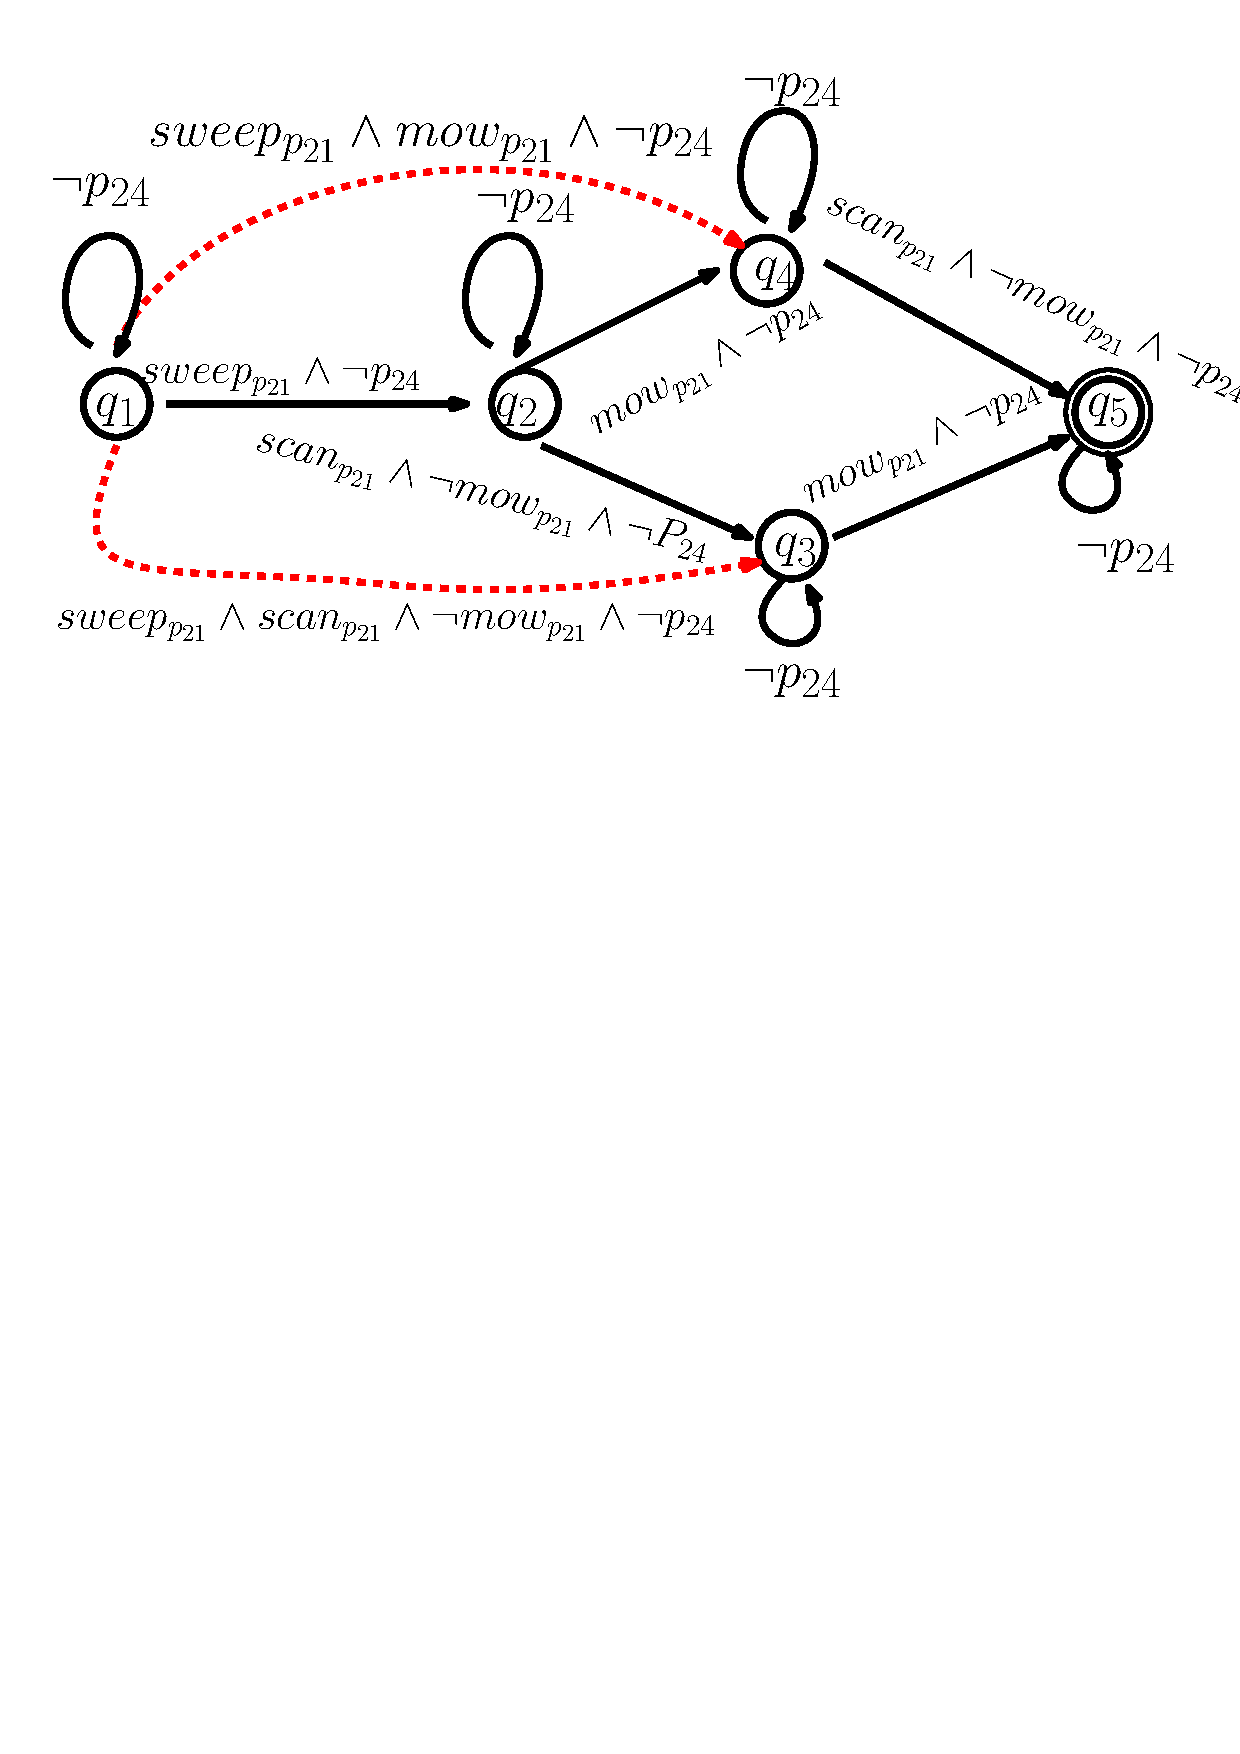
\includegraphics[scale=0.35]{figures/example_decomposable.pdf}
\caption{
Example of decomposable transitions.
Any transition in red dashed line are all
decomposable satisfied by Def.~\ref{def:decomposable-transition}.}
\label{fig:example_decomposable}
\end{figure}
%========================================

\begin{example}\label{eq:prune-nba}
The NBA~$\mathcal{B}_{\varphi}$ associated with the task formula in~\eqref{example:task}
has $707$ states and $16044$ edges with more than $1.29\times10^7$ accepting \textcolor{blue}{\emph{word}s},
translated via~\citep{gastin2001fast}.
After the pruning process described above, the pruned automaton~$\mathcal{B}^{-}_{\varphi}$
has $707$ states and $2423$ edges with $174469$ accepting \emph{words}. This step reduces $84.9\%$ edges and $98.6\%$
accepting \emph{words}.
\hfill $\blacksquare$
\end{example}
